\documentclass{standalone}
\usepackage{tikz}
\usetikzlibrary{patterns, positioning}
\usepackage[sfdefault]{ClearSans} %% option 'sfdefault' activates Clear Sans as the default text font
\usepackage[T1]{fontenc}

\begin{document}
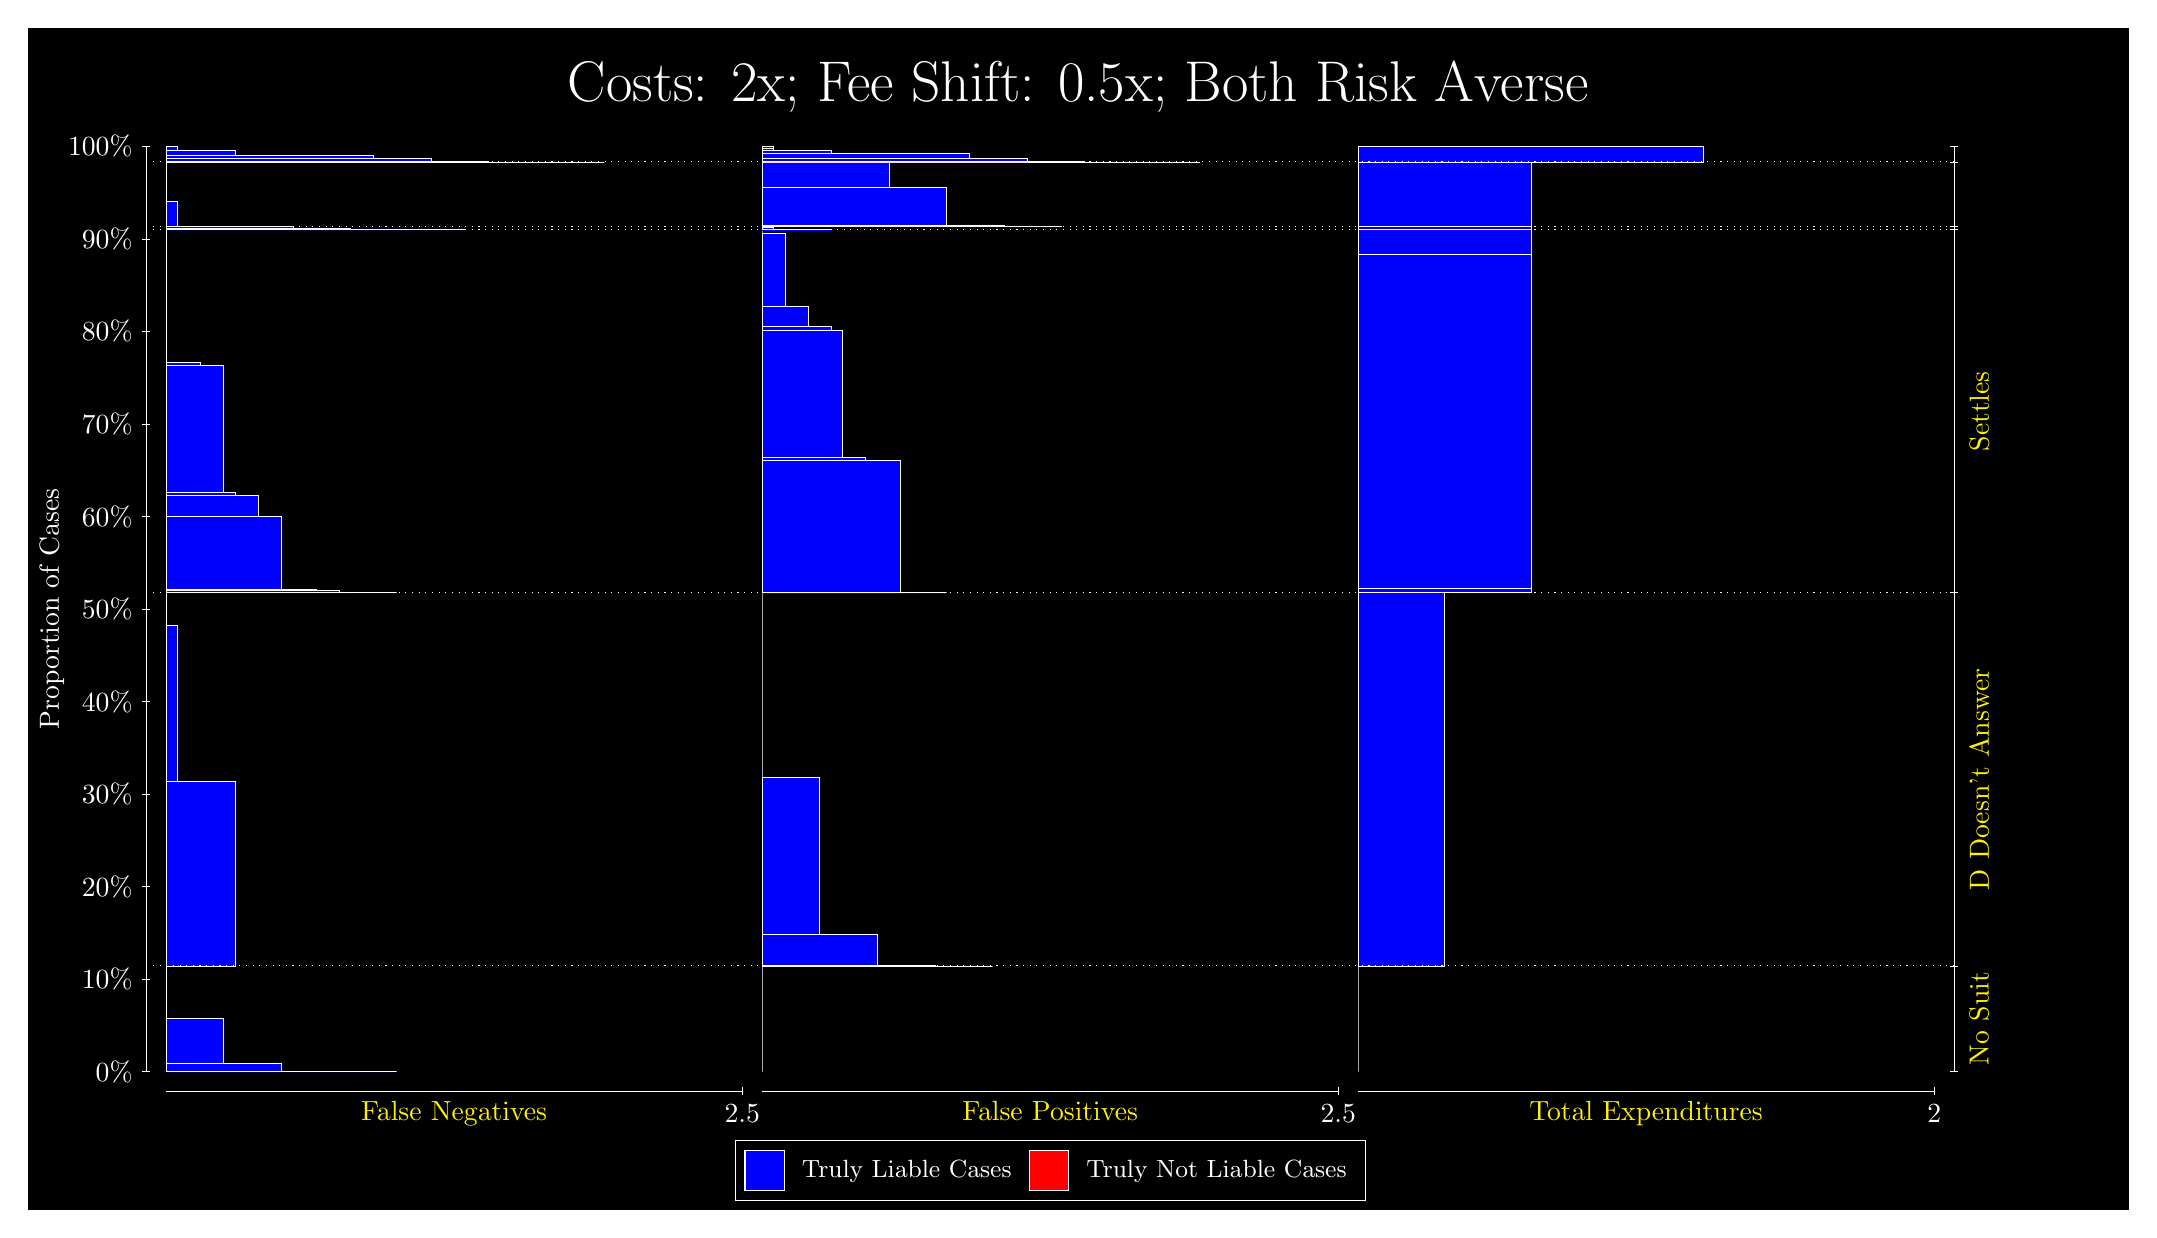
\begin{tikzpicture}
\draw[fill=black] (0,0) rectangle (26.667,15);
\draw[text=white] (0,13.5) rectangle (26.667,15) node[midway] {\huge Costs: 2x; Fee Shift: 0.5x; Both Risk Averse};
\draw[white, very thin] (1.5,1.75) -- (1.5,13.5);
\node[rotate=90, text=white, anchor=center] at (0.3, 7.625) {Proportion of Cases};
\draw[white, very thin] (1.45,1.75) -- (1.55,1.75);
\node[text=white, anchor=east] at (1.45, 1.75) {0\%};
\draw[white, very thin] (1.45,2.925) -- (1.55,2.925);
\node[text=white, anchor=east] at (1.45, 2.925) {10\%};
\draw[white, very thin] (1.45,4.1) -- (1.55,4.1);
\node[text=white, anchor=east] at (1.45, 4.1) {20\%};
\draw[white, very thin] (1.45,5.275) -- (1.55,5.275);
\node[text=white, anchor=east] at (1.45, 5.275) {30\%};
\draw[white, very thin] (1.45,6.45) -- (1.55,6.45);
\node[text=white, anchor=east] at (1.45, 6.45) {40\%};
\draw[white, very thin] (1.45,7.625) -- (1.55,7.625);
\node[text=white, anchor=east] at (1.45, 7.625) {50\%};
\draw[white, very thin] (1.45,8.8) -- (1.55,8.8);
\node[text=white, anchor=east] at (1.45, 8.8) {60\%};
\draw[white, very thin] (1.45,9.975) -- (1.55,9.975);
\node[text=white, anchor=east] at (1.45, 9.975) {70\%};
\draw[white, very thin] (1.45,11.15) -- (1.55,11.15);
\node[text=white, anchor=east] at (1.45, 11.15) {80\%};
\draw[white, very thin] (1.45,12.325) -- (1.55,12.325);
\node[text=white, anchor=east] at (1.45, 12.325) {90\%};
\draw[white, very thin] (1.45,13.5) -- (1.55,13.5);
\node[text=white, anchor=east] at (1.45, 13.5) {100\%};

\draw[white, very thin] (24.457,1.75) -- (24.457,13.5);
\draw[white, very thin] (24.407,1.75) -- (24.507,1.75);
\node[anchor=west] at (24.407, 1.75) {};
\draw[white, very thin] (24.407,3.0926) -- (24.507,3.0926);
\node[anchor=west] at (24.407, 3.0926) {};
\draw[white, very thin] (24.407,7.8303) -- (24.507,7.8303);
\node[anchor=west] at (24.407, 7.8303) {};
\draw[white, very thin] (24.407,12.441) -- (24.507,12.441);
\node[anchor=west] at (24.407, 12.441) {};
\draw[white, very thin] (24.407,12.484) -- (24.507,12.484);
\node[anchor=west] at (24.407, 12.484) {};
\draw[white, very thin] (24.407,13.303) -- (24.507,13.303);
\node[anchor=west] at (24.407, 13.303) {};
\draw[white, very thin] (24.407,13.5) -- (24.507,13.5);
\node[anchor=west] at (24.407, 13.5) {};

\draw[white, very thin, fill=blue] (1.75,1.75) rectangle (4.6775,1.75);
\draw[white, very thin, fill=blue] (1.75,1.75) rectangle (3.9457,1.7509);
\draw[white, very thin, fill=blue] (1.75,1.7509) rectangle (3.2138,1.8574);
\draw[white, very thin, fill=blue] (1.75,1.8574) rectangle (2.4819,2.4222);
\draw[white, very thin, fill=red] (1.75,2.4222) rectangle (1.75,2.4222);
\draw[white, very thin, fill=blue] (1.75,2.4222) rectangle (1.75,3.0926);
\draw[white, very thin, fill=blue] (1.75,3.0926) rectangle (2.6283,5.4388);
\draw[white, very thin, fill=blue] (1.75,5.4388) rectangle (1.8964,7.4237);
\draw[white, very thin, fill=red] (1.75,7.4237) rectangle (1.75,7.4237);
\draw[white, very thin, fill=blue] (1.75,7.4237) rectangle (1.75,7.8303);
\draw[white, very thin, fill=blue] (1.75,7.8303) rectangle (4.6775,7.8303);
\draw[white, very thin, fill=blue] (1.75,7.8303) rectangle (4.3848,7.8303);
\draw[white, very thin, fill=blue] (1.75,7.8303) rectangle (4.092,7.8303);
\draw[white, very thin, fill=blue] (1.75,7.8303) rectangle (3.9457,7.8608);
\draw[white, very thin, fill=blue] (1.75,7.8608) rectangle (3.6529,7.8731);
\draw[white, very thin, fill=blue] (1.75,7.8731) rectangle (3.3602,7.8752);
\draw[white, very thin, fill=blue] (1.75,7.8752) rectangle (3.2138,8.806);
\draw[white, very thin, fill=blue] (1.75,8.806) rectangle (2.921,9.0624);
\draw[white, very thin, fill=blue] (1.75,9.0624) rectangle (2.6283,9.1054);
\draw[white, very thin, fill=blue] (1.75,9.1054) rectangle (2.4819,10.718);
\draw[white, very thin, fill=blue] (1.75,10.718) rectangle (2.1891,10.757);
\draw[white, very thin, fill=blue] (1.75,10.757) rectangle (1.8964,10.763);
\draw[white, very thin, fill=red] (1.75,10.763) rectangle (1.75,10.763);
\draw[white, very thin, fill=blue] (1.75,10.763) rectangle (1.75,12.441);
\draw[white, very thin, fill=blue] (1.75,12.441) rectangle (5.5558,12.441);
\draw[white, very thin, fill=blue] (1.75,12.441) rectangle (4.8239,12.441);
\draw[white, very thin, fill=blue] (1.75,12.441) rectangle (4.092,12.456);
\draw[white, very thin, fill=blue] (1.75,12.456) rectangle (3.3602,12.483);
\draw[white, very thin, fill=blue] (1.75,12.483) rectangle (2.6283,12.484);
\draw[white, very thin, fill=red] (1.75,12.484) rectangle (1.75,12.484);
\draw[white, very thin, fill=blue] (1.75,12.484) rectangle (2.6283,12.488);
\draw[white, very thin, fill=blue] (1.75,12.488) rectangle (1.8964,12.804);
\draw[white, very thin, fill=red] (1.75,12.804) rectangle (1.75,12.804);
\draw[white, very thin, fill=blue] (1.75,12.804) rectangle (1.75,13.303);
\draw[white, very thin, fill=blue] (1.75,13.303) rectangle (7.3123,13.303);
\draw[white, very thin, fill=blue] (1.75,13.303) rectangle (6.5805,13.303);
\draw[white, very thin, fill=blue] (1.75,13.303) rectangle (5.8486,13.305);
\draw[white, very thin, fill=blue] (1.75,13.305) rectangle (5.1167,13.349);
\draw[white, very thin, fill=blue] (1.75,13.349) rectangle (4.8239,13.349);
\draw[white, very thin, fill=blue] (1.75,13.349) rectangle (4.3848,13.39);
\draw[white, very thin, fill=blue] (1.75,13.39) rectangle (4.092,13.39);
\draw[white, very thin, fill=blue] (1.75,13.39) rectangle (3.6529,13.39);
\draw[white, very thin, fill=blue] (1.75,13.39) rectangle (3.3602,13.392);
\draw[white, very thin, fill=blue] (1.75,13.392) rectangle (2.921,13.392);
\draw[white, very thin, fill=blue] (1.75,13.392) rectangle (2.6283,13.392);
\draw[white, very thin, fill=blue] (1.75,13.392) rectangle (2.6283,13.45);
\draw[white, very thin, fill=blue] (1.75,13.45) rectangle (1.8964,13.451);
\draw[white, very thin, fill=blue] (1.75,13.451) rectangle (1.8964,13.496);
\draw[white, very thin, fill=red] (1.75,13.496) rectangle (1.75,13.496);
\draw[white, very thin, fill=blue] (1.75,13.496) rectangle (1.75,13.5);
\draw[white, very thin, fill=red] (9.3189,1.75) rectangle (9.3189,1.75);
\draw[white, very thin, fill=blue] (9.3189,1.75) rectangle (9.3189,3.0926);
\draw[white, very thin, fill=red] (9.3189,3.0926) rectangle (12.246,3.0926);
\draw[white, very thin, fill=blue] (9.3189,3.0926) rectangle (12.246,3.0926);
\draw[white, very thin, fill=blue] (9.3189,3.0926) rectangle (11.515,3.1041);
\draw[white, very thin, fill=blue] (9.3189,3.1041) rectangle (10.783,3.4991);
\draw[white, very thin, fill=blue] (9.3189,3.4991) rectangle (10.051,5.4841);
\draw[white, very thin, fill=blue] (9.3189,5.4841) rectangle (9.3189,7.8303);
\draw[white, very thin, fill=red] (9.3189,7.8303) rectangle (11.661,7.8303);
\draw[white, very thin, fill=blue] (9.3189,7.8303) rectangle (11.661,7.8303);
\draw[white, very thin, fill=red] (9.3189,7.8303) rectangle (11.368,7.8303);
\draw[white, very thin, fill=blue] (9.3189,7.8303) rectangle (11.368,7.8304);
\draw[white, very thin, fill=red] (9.3189,7.8304) rectangle (11.075,7.8304);
\draw[white, very thin, fill=blue] (9.3189,7.8304) rectangle (11.075,9.5081);
\draw[white, very thin, fill=blue] (9.3189,9.5081) rectangle (10.929,9.5145);
\draw[white, very thin, fill=blue] (9.3189,9.5145) rectangle (10.636,9.5529);
\draw[white, very thin, fill=blue] (9.3189,9.5529) rectangle (10.344,11.166);
\draw[white, very thin, fill=blue] (9.3189,11.166) rectangle (10.197,11.209);
\draw[white, very thin, fill=blue] (9.3189,11.209) rectangle (9.9044,11.465);
\draw[white, very thin, fill=blue] (9.3189,11.465) rectangle (9.6116,12.396);
\draw[white, very thin, fill=blue] (9.3189,12.396) rectangle (9.4652,12.398);
\draw[white, very thin, fill=blue] (9.3189,12.398) rectangle (9.3189,12.441);
\draw[white, very thin, fill=red] (9.3189,12.441) rectangle (10.197,12.441);
\draw[white, very thin, fill=blue] (9.3189,12.441) rectangle (10.197,12.442);
\draw[white, very thin, fill=blue] (9.3189,12.442) rectangle (9.4652,12.469);
\draw[white, very thin, fill=blue] (9.3189,12.469) rectangle (9.3189,12.484);
\draw[white, very thin, fill=red] (9.3189,12.484) rectangle (13.125,12.484);
\draw[white, very thin, fill=blue] (9.3189,12.484) rectangle (13.125,12.484);
\draw[white, very thin, fill=blue] (9.3189,12.484) rectangle (12.393,12.497);
\draw[white, very thin, fill=blue] (9.3189,12.497) rectangle (11.661,12.983);
\draw[white, very thin, fill=blue] (9.3189,12.983) rectangle (10.929,13.299);
\draw[white, very thin, fill=blue] (9.3189,13.299) rectangle (10.197,13.303);
\draw[white, very thin, fill=red] (9.3189,13.303) rectangle (14.881,13.303);
\draw[white, very thin, fill=blue] (9.3189,13.303) rectangle (14.881,13.303);
\draw[white, very thin, fill=red] (9.3189,13.303) rectangle (14.149,13.303);
\draw[white, very thin, fill=blue] (9.3189,13.303) rectangle (14.149,13.303);
\draw[white, very thin, fill=red] (9.3189,13.303) rectangle (13.417,13.303);
\draw[white, very thin, fill=blue] (9.3189,13.303) rectangle (13.417,13.307);
\draw[white, very thin, fill=red] (9.3189,13.307) rectangle (12.686,13.307);
\draw[white, very thin, fill=blue] (9.3189,13.307) rectangle (12.686,13.353);
\draw[white, very thin, fill=blue] (9.3189,13.353) rectangle (11.954,13.411);
\draw[white, very thin, fill=red] (9.3189,13.411) rectangle (11.661,13.411);
\draw[white, very thin, fill=blue] (9.3189,13.411) rectangle (11.661,13.411);
\draw[white, very thin, fill=blue] (9.3189,13.411) rectangle (11.222,13.412);
\draw[white, very thin, fill=red] (9.3189,13.412) rectangle (10.929,13.412);
\draw[white, very thin, fill=blue] (9.3189,13.412) rectangle (10.929,13.413);
\draw[white, very thin, fill=blue] (9.3189,13.413) rectangle (10.49,13.413);
\draw[white, very thin, fill=blue] (9.3189,13.413) rectangle (10.197,13.453);
\draw[white, very thin, fill=red] (9.3189,13.453) rectangle (10.197,13.453);
\draw[white, very thin, fill=blue] (9.3189,13.453) rectangle (10.197,13.453);
\draw[white, very thin, fill=blue] (9.3189,13.453) rectangle (9.758,13.453);
\draw[white, very thin, fill=blue] (9.3189,13.453) rectangle (9.4652,13.479);
\draw[white, very thin, fill=blue] (9.3189,13.479) rectangle (9.4652,13.497);
\draw[white, very thin, fill=blue] (9.3189,13.497) rectangle (9.3189,13.5);
\draw[white, very thin, fill=red] (16.888,1.75) rectangle (16.888,1.75);
\draw[white, very thin, fill=blue] (16.888,1.75) rectangle (16.888,3.0926);
\draw[white, very thin, fill=red] (16.888,3.0926) rectangle (17.986,3.0926);
\draw[white, very thin, fill=blue] (16.888,3.0926) rectangle (17.986,7.8303);
\draw[white, very thin, fill=red] (16.888,7.8303) rectangle (19.083,7.8303);
\draw[white, very thin, fill=blue] (16.888,7.8303) rectangle (19.083,7.8819);
\draw[white, very thin, fill=red] (16.888,7.8819) rectangle (19.083,7.8819);
\draw[white, very thin, fill=blue] (16.888,7.8819) rectangle (19.083,12.134);
\draw[white, very thin, fill=red] (16.888,12.134) rectangle (19.083,12.134);
\draw[white, very thin, fill=blue] (16.888,12.134) rectangle (19.083,12.441);
\draw[white, very thin, fill=red] (16.888,12.441) rectangle (19.083,12.441);
\draw[white, very thin, fill=blue] (16.888,12.441) rectangle (19.083,12.484);
\draw[white, very thin, fill=red] (16.888,12.484) rectangle (19.083,12.484);
\draw[white, very thin, fill=blue] (16.888,12.484) rectangle (19.083,13.303);
\draw[white, very thin, fill=red] (16.888,13.303) rectangle (21.279,13.303);
\draw[white, very thin, fill=blue] (16.888,13.303) rectangle (21.279,13.5);
\draw[white, dotted] (1.5,3.0926) -- (24.457,3.0926);
\draw[white, dotted] (1.5,7.8303) -- (24.457,7.8303);
\draw[white, dotted] (1.5,12.441) -- (24.457,12.441);
\draw[white, dotted] (1.5,12.484) -- (24.457,12.484);
\draw[white, dotted] (1.5,13.303) -- (24.457,13.303);
\draw[white, very thin] (1.75,1.5) -- (9.0689,1.5);
\node[text=yellow, anchor=north] at (5.4094, 1.5) {False Negatives};
\draw[white, very thin] (9.0689,1.45) -- (9.0689,1.55);
\node[text=white, anchor=north] at (9.0689, 1.45) {2.5};

\draw[white, very thin] (9.3189,1.5) -- (16.638,1.5);
\node[text=yellow, anchor=north] at (12.978, 1.5) {False Positives};
\draw[white, very thin] (16.638,1.45) -- (16.638,1.55);
\node[text=white, anchor=north] at (16.638, 1.45) {2.5};

\draw[white, very thin] (16.888,1.5) -- (24.207,1.5);
\node[text=yellow, anchor=north] at (20.547, 1.5) {Total Expenditures};
\draw[white, very thin] (24.207,1.45) -- (24.207,1.55);
\node[text=white, anchor=north] at (24.207, 1.45) {2};

\node[text=yellow, centered, rotate=90] at (24.777, 2.4213) {No Suit};
\node[text=yellow, centered, rotate=90] at (24.777, 5.4614) {D Doesn't Answer};
\node[text=yellow, centered, rotate=90] at (24.777, 10.136) {Settles};




\draw (12.978300999999998,1.5) node[draw=none] (baseCoordinate) {};
\begin{scope}[align=center]
        \matrix[scale=0.5, draw=white, below=0.5cm of baseCoordinate, nodes={draw}, column sep=0.1cm]{
            \node[rectangle, draw, minimum width=0.5cm, minimum height=0.5cm, fill=blue] {}; &
            \node[draw=none, font=\small, text=white] (B) {Truly Liable Cases}; &
            \node[rectangle, draw, minimum width=0.5cm, minimum height=0.5cm, fill=red] {}; &
            \node[draw=none, font=\small, text=white] (B) {Truly Not Liable Cases}; \\
            };
\end{scope}

\end{tikzpicture}
\end{document}